\documentclass{article}
\usepackage[utf8]{inputenc}
\usepackage{graphicx}
\usepackage{float}
\usepackage{svg}

\usepackage{amssymb}
\usepackage{amsmath}

\title{Multi Agent System approach. A road to robot cooperation}
\author{}
\date{February 2020}

\begin{document}


\begin{titlepage}
	
	\hspace{0.071cm}
\includegraphics[width=0.5\textwidth]{img/logo_CFIS.jpg}\hspace{0.2cm}
	
\includegraphics[scale=0.25]{img/hcrl.png}	
	\par\vspace{0.4cm}
	\hspace{0.13cm}
\includegraphics[scale=0.061125]{img/logo_FIB.jpg}\par \vspace{0.3cm}
	
\includegraphics[scale=0.25]{img/logo_FME.jpg}\par\vspace{1cm}
	\centering
	\vspace{1cm}
	{\scshape\LARGE Bachleor Thesis \par}
	\vspace{2cm}
	{\scshape\LARGE \textbf{Multi-Agent Systems, a road to robot coperation} \par}
	\vspace{1.5cm}
	{\Large Jordi Bosch \par}
	\vspace{1cm}
	\begin{flushleft}
	{\textbf{Degrees:}\par}
	{Degree in Computer Science FIB \par}
	{Degree in Mathematics FME \par }
	
	{\textbf{Advisors:}\par \par }
	{Dra. Maria José Serna Iglesias \par}
	{Dr. Luis Sentis Álvarez}
	\end{flushleft}
	\vfill

	{\large February 2020}
\end{titlepage}
\begin{center}
\section{Abstract}

\end{center}

Robots are becoming more and more involved in everyday tasks, helping people to clean, cook and manipulate all kinds of objects. Most of the time we picture ourselves one robot doing the different tasks, but, what would happen if we had several robots trying to do the same job?\newline\newline
In this thesis we focus our goal in robot cooperation. Our objective is to explore how can different robots learn together in order to perform optimally a set of tasks. This may have lots of applications in the real world since we can have a set of heterogeneous robots, for the sake of simplicity(a drone and a terrestial robot) each one beneficing from the information the other one perceives and exploring an unkown terrain more fast.
\newline \newline
In this thesis we have set up a work space in which we are  able to deeply study the performance and the learning of two robots. We will face the problems that arise in the learning and will keep track of the solutions that we come up with.

\newpage

\tableofcontents
\maketitle

\section{Introduction}
\section{Special thanks}
This project wouldn't have been possible without ma nigros. My negro Erik Ferrando, my ciervo Marc Esquerranus il hombre annus and my Reggeatonero del MIT Eric Sipote.
\section{Multi Agent Systems:an overview}
\section{Reinforcement Learning aproach for 
coordination}
\subsection{Theoretical formulation}
Inside the machine learning methods we can find 3 different big types:
\begin{itemize}
\item Supervised Learning. Inferring a regression or classification through a labeled trainging data
\item Unsupervised Learning. Inferring from datasets without labels.
\item Reinforcement Learning. Study how an agent must behave in order to maximize the cumulative reward. 
\end{itemize}  
Thiss last type is what we will exploitf. It is the best scenario when we have an idea of which actions are "good" and "bad" and we want to maximize the goodness of our agent. Let's go through the theory and algorithms used in this paradigm.
\newline
In our framework we will have an agent that does the decision making and everything out of the agent is the environmnent. The environment is responsible to offer a response for each action the agent takes, providing a new environment state and the reward for the action the agent took (See figure 1). They interact continuouslly.
\newline
Lets state this in a more formal way.
We have a set of states $\mathcal{S}$. Initially our agent starts at a determined state $ s \subseteq \mathcal{S}$. For the sake of simplicity lets denote $S_{t}$ the state the Agent is at the $t$ timestep. For each state $S_{t}$ we have a set of actions the agent can take $A(S_{t})$. Once the agent has chosen an action the environment returns a new state $S_{t+1}$ and a reward $R_{t+1}$. \newline
\newline
\begin{figure}[H]
\centering 
$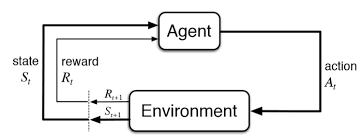
\includegraphics[scale=0.7]{agent_environment.png}$
\caption{Agent-Environment diagram}
\end{figure}
The agent learns a policy $\pi(a|s)$ that at every state assigns a probability of each action available in this state of being chosen. This policy keeps changing over experience and our goal is to build a policy that maximizes the cumulated reward from the initial to the terminal state. 
\newline
How can we maximize the total reward? 
\newline Lets denote $G_{t} = R_{t+1} + R_{t+2} + R_{t+3} + \dots $ If our interactions go over infinity we will use the discounted return in order to make them finite.\newline
$G_{t} = R_{t+1} + \gamma R_{t+2} + \gamma^{2} R_{t+3} + \dots + R_{T} = \sum_{i = 0}^{\infty}\gamma^{i} R_{t+1+i} $ choosing a $\gamma < 1$. If the rewards are bounded we can easily see this series is convergent. We chose $\gamma < \delta < 1$ and we see that $$\lim_{i\to\infty}\frac{\delta^{i}}{\gamma^{i}*R_{t+1+i}} = \lim_{i\to\infty}(\frac{\delta}{\gamma})^{i} * \frac{1}{R_{t+1+i}} = \infty$$ since it is the exponential of a number bigger than 1 multiplied by a bounded series. That means that from a point of the series the second series is bigger than the first, since the second series is the geometric series of $\delta$ and we know it is convergent, so it is the first one.
\newline
The parameter $\gamma$ can also be used in non infinite tasks. In a sense it is a way of weighting the rewards. If $\gamma$ is close to $ 1$ we want each reward to count the same. If $\gamma$ is close to $0$ we want the first rewards to count more than the next ones in the task.
\subsection{Markov Property}
The election of our states will be very important. We want to choose as states some variables that give us enough information in order to sintesize all the information we need for our problem. For example, in a chess game, a good state variable is the position of all the pieces(the board itself) since it ofers all the information we need in order to know what action to choose next. It must be clear that there is some information lost in this representation. We don't know how the pieces arranged themselves to the positions that are in this moment.\newline
A state signal that suceeds at storing all relevant information is said to have the Markov property.\newline
We now define the Markov property in the Reinforcement Learning paradigm. We say that a state variable has the Markov propery if:\newline
$$Pr(R_{t+1},S_{t+1}|S_{0},A_{0},\dots,S_{t},A_{t}) = Pr(R_{t+1},S_{t+1}|S_{t},A_{t})$$ that is, the probability of going to the next state and geting a determined reward depends only in the previous state and action. That means that our state signal is really good since it is possible to sintesize all the past information into a state. This will simplify a lot lots of calculations.\newline
A problem with the Markov property is called a Markov Decision Problem(MDP). And this are the types of problems I will be working on. If we know $$p(s',r|s,a)$$ we have the problem completely specified. In this scenario we introduce value functions.\newline
$$v_{\pi}(s) = \mathbb{E}_{\pi}[G_{t}|S_{t} = s] = \mathbb{E}[\sum_{k = 0}^{\infty}\gamma^{k}R_{t+k+1}|S_{t} = s]$$ The value function of a state given a policy $\pi$ is the Expectation of the cumulated reward starting from this state following policy $\pi$. We also define: 
$$q_{\pi}(s,a) = \mathbb{E}_{\pi}[G_{t}|S_{t} = s, A = a] = \mathbb{E}[\sum_{k = 0}^{\infty}\gamma^{k}R_{t+k+1}|S_{t} = s, A = a]$$ which is the Expectation starting from state s and taking firstly action a. At this point we can proceed in two ways for trying to estimate $v_{\pi}(s)$ and $q_{\pi}(s,a)$. First of all we can do it over experience. We can keep track of the results and then doing an average. We know, by the law of large numbers that it would converge to the true value. Otherwise, we can try to exploit the recursive nature of the equation:\newline
\begin{equation}
	\begin{aligned}
	v_{\pi}(s) = {}&\mathbb{E}_{\pi}[G_{t}|S_{t} = s] \\
	={}& \mathbb{E}_{\pi}[\sum_{k = 0}^{\infty}\gamma^{k}R_{t+k+1}|S_{t} = s] \\
	= {}& \mathbb{E}_{\pi}[R_{t+1} + \gamma \sum_{k = 0}			^{\infty}\gamma^{k} R_{t+k+2}|S_{t} = s] \\	
	= {}& \sum_{a}^{}\pi(a|s) \sum_{s'}^{}	\sum_{r}^{}p(s',r|s,a)[r + \gamma \mathbb{E}_{\pi}[\sum_{k = 0}			^{\infty}\gamma^{k} R_{t+k+2}|S_{t+1} = s']]\\
	= {}& \sum_{a}^{}\pi(a|s) \sum_{s'}^{r}p(s',r|s,a)[r + \gamma v_{\pi}(s')]
	\end{aligned}	
\end{equation}
We get one equation of as many unkowns as states there are. We can do a similar reasoning for each state and get $n$ equations and $n$ unkowns. We can solve this system of equations using iterative methods since the number of states can be extremelly large in most problems. Solving, for each policy we get the value function of each state.\newline
How can we keep improving our policy to make it the optimal?\newline
We want to obtain the value functions of the optimal policy. But first of all we need a method for improving a policy. By improving a policy we try to find a different policy that yields a highest value functions for every state. That is the optimal policy $\pi ^{*}$ is the one that $v_{\pi^{*}}(s) \geq v_{\pi}(s) \forall s \forall \pi$.\newline
For improving an existing policy we can choose the action that yields highest reward at each step. That is given a policy $\pi$, we chose our improved policy $\pi'$ to be at a given state $s$,  $\pi'(s) = $argmax $q_{\pi}(s,a)$. \newline That is, we choose the action with highest expected value for the given policy. We keep iterating for each state until the new policy becomes stable.(Insert image). We keep doing that until we arrive at the optimal policy. 
Now that we have a method for finding the optimal policy and the value functions at the optimal policy, we would think that we can solve every problem that we ran into. The problem with that though is that in lots of problems it becomes impractical or impossible to know beforehand all the transition values $p(s',r|s,a)$.\newline
That makes this approach sometimes useless and we have to think of some variants. 
\subsection{Temporal Difference Learning}
This methods blend between Monte Carlo methods(just averaging the samples) and DP methods(updating the values at each timestep). The idea is fairly simple, at each state we will update the value function of the state $s$, $$V(S_{t}) = V(S_{t}) + \alpha * (G_{t} - V(S_{t}))$$That is we update the value towards the true value being $G_{t}$ an unbiased estimator of $V(S_{t})$. In our case the update algorithm will be:\newline
$$V(S_{t}) \leftarrow V(S_{t}) + \alpha (r + \gamma V(s') - V(s))$$ Being $r$ and $V(s')$ the reward and new state following the policy from state $s$.This will be one of our common points in all the algorithms we implement.\newline
\subsubsection{Sarsa Algorithm}
\subsubsection{Q Learning Algorithm}
\subsubsection{Eligibility Traces}

\section{Results}
\section{Future Work}
\end{document}
